\section{Поняття бінарного відношення. Відношення порядку. Функціональне відношення}

\begin{definition}
    \textbf{Бінарне відношення} --- це деяка підмножина декартового добутку
    двох множин, тобто довільна множина упорядкованих пар:

    $R \subset X \times Y$, $R \subset \{(x,y): x \in X \wedge y \in Y\}$.
\end{definition}

Запис: $(x,y) \in R$, або $xRy$, означає, що $x$ зв'язаний з $y$
відношенням $R$.

Множини перших та других елементів упорядкованих пар, що утворюють деяке відношення,
це --- \textbf{область визначення} і \textbf{область значень} цього відношення
відповідно.

Якщо $R \subset X^2$ (тобто $R \subset X \times X$), то говорять, що відношення
$R$ \textit{задано на множині $X$}.

\begin{definition}
    Відношення $R \subset X^2$ --- це \textbf{відношення часткового порядку}, якщо
    виконуються наступні властивості:
    \begin{enumerate}
        \item $\forall x \in X \: xRx$ (рефлексивність)
        \item $(xRy \wedge yRx) \Rightarrow x = y$ (антисиметричність)
        \item $(xRy \wedge yRz) \Rightarrow xRz$ (транзитивність)
    \end{enumerate}
\end{definition}

Множина $X$, на якій введено відношення часткового порядку $R \subset x^2$
є частково упорядкованою.

Для такого відношення, запис $xRy$ означає, що $y$ слідує за $x$, або $x$ передує $y$
(де $x$ та $y$ --- елементи множини $X$).

\begin{example}
    Відношення частково порядку на $N$:

    \begin{enumerate}
        \item $R$: "$a$ є дільником $b$".
        \item $R$: "$a$ менше рівно $b$".
    \end{enumerate}
\end{example}

Нехай $R \subset X^2$ --- відношення часткового порядку на $X$. Якщо будь які два елементи
$x$ та $y$ множини $X$ при цьому порівнюємі (тобто $xRy$ або $yRx$), то таке відношення ---
це \textbf{відношення порядку}, а множина $X$ --- \textbf{упорядкована множина}.

\begin{example}~

    \begin{enumerate}
        \item $R$: "$a$ менше рівно $b$".
        \item $R$: "$a$ є дільником $b$" --- не відношення порядку, бо наприклад числа 2 та 3
            не є порівнюваними.
    \end{enumerate}
\end{example}

Відношення $R \subset X \times Y$ --- це \textbf{функціональне відношення}, якщо 
$(xRy_1 \wedge xRy_2) \Rightarrow y_1 = y_2$, тобто якщо воно не містить різних пар з
однаковими першими елементами.

\begin{center}
    \begin{tikzpicture}[scale=0.5]
        \draw (2,3) ellipse (2cm and 3cm);
        \draw (8,3) ellipse (2cm and 3cm);
        %\draw[gray, dashed] (0,0) grid (10,6);

        \draw (0,4) node[above left]{X};
        \draw (10,4) node[above right]{Y};

        \filldraw[black] (2,5) circle (2pt);

        \filldraw[black] (3,4) circle (2pt);
        \filldraw[black] (7,5) circle (2pt);
        \filldraw[black] (9,4) circle (2pt);
        \draw[thick] (3,4) -- (7,5);
        \draw[-stealth, thick] (3,4) -- (5,4.5);
        \draw[thick] (3,4) -- (9,4);
        \draw[-stealth, thick] (3,4) -- (5,4);

        \filldraw[black] (1.5,3.5) circle (2pt);
        \filldraw[black] (8.5,2.5) circle (2pt);
        \draw[thick] (1.5,3.5) -- (8.5,2.5);
        \draw[-stealth, thick] (1.5,3.5) -- (5,3);

        \filldraw[black] (3,1.5) circle (2pt);
        \filldraw[black] (7,3) circle (2pt);
        \draw[thick] (3,1.5) -- (7,3);
        \draw[-stealth, thick] (3,1.5) -- (5,2.25);

        \filldraw[black] (1,2) circle (2pt);

        \filldraw[black] (2,1) circle (2pt);
        \filldraw[black] (8,1) circle (2pt);
        \draw[-stealth, thick] (2,1) -- (5,1);
        \draw[thick] (2,1) -- (8,1);

        \filldraw[black] (9,3) circle (2pt);

        \draw (5,-1) node{відношення не функціональне};
    \end{tikzpicture}
    \begin{tikzpicture}[scale=0.5]
        \draw (2,3) ellipse (2cm and 3cm);
        \draw (8,3) ellipse (2cm and 3cm);
        %\draw[gray, dashed] (0,0) grid (10,6);

        \draw (0,4) node[above left]{X};
        \draw (10,4) node[above right]{Y};

        \filldraw[black] (1.5,5) circle (2pt);
        \filldraw[black] (8.5,5) circle (2pt);
        \draw[thick] (1.5,5) -- (8.5,5);
        \draw[-stealth, thick] (1.5,5) -- (5,5);
        
        \filldraw[black] (3,4) circle (2pt);
        \filldraw[black] (2,2) circle (2pt);
        \filldraw[black] (8,4) circle (2pt);
        \draw[thick] (3,4) -- (8,4);
        \draw[-stealth, thick] (3,4) -- (5,4);
        \draw[thick] (2,2) -- (8,4);
        \draw[-stealth, thick] (2,2) -- (5,3);

        \filldraw[black] (2.25,1) circle (2pt);
        \filldraw[black] (8.25,2) circle (2pt);
        \draw[thick] (2.25,1) -- (8.25,2);
        \draw[-stealth, thick] (2.25,1) -- (5.25,1.5);

        \filldraw[black] (1,3) circle (2pt);

        \filldraw[black] (9,3.5) circle (2pt);

        \filldraw[black] (7.7,1) circle (2pt);

        \draw (5,-1) node{відношення функціональне};
    \end{tikzpicture}
\end{center}

\section{Відображення(функція). Образ та прообраз множини. Класифікація відображень}

Нехай $R \subset X \times Y$ --- функціональне відношення. Якщо множина $X$
співпадає з областю візначення цього відношення (тобто $X$ утворено першими
елементами тільки тих упорядкованих пар, які утворюють відношення $R$), то це
функціональне відношення --- це \textit{відображення функції із $X$ \underline{\underline{в}} $y$}

Таким чином, якщо відношення $R \subset X \times Y$ це функція, то для кожного
елемента $x$ із $X$ існує, щей при тому єдиний, елемент $y$ із $Y$, такий, що
$xRy$.

\begin{equation*}
    R \subset X \times Y \text{ - функція } \Rightarrow \forall x \in X \quad \exists! y \in Y: xRy
\end{equation*}

Якщо не тільки $X$ співпадає з областю визначення, а й $Y$ співпадає з множиною
значень, то це відображення --- це \textit{відображення із $X$
\underline{\underline{на}} $y$}

\begin{center}
    \begin{tikzpicture}[scale=0.5]
        \draw (2,3) ellipse (2cm and 3cm);
        \draw (8,3) ellipse (2cm and 3cm);
        %\draw[gray, dashed] (0,0) grid (10,6);

        \draw (0,5) node[above]{X};
        \draw (10,5) node[above]{Y};

        \filldraw[black] (1.5,5) circle (2pt);
        \filldraw[black] (8.5,5) circle (2pt);
        \draw[thick] (1.5,5) -- (8.5,5);
        \draw[-stealth, thick] (1.5,5) -- (5,5);
        
        \filldraw[black] (3,4) circle (2pt);
        \filldraw[black] (2,2) circle (2pt);
        \filldraw[black] (8,4) circle (2pt);
        \draw[thick] (3,4) -- (8,4);
        \draw[-stealth, thick] (3,4) -- (5,4);
        \draw[thick] (2,2) -- (8,4);
        \draw[-stealth, thick] (2,2) -- (5,3);

        \filldraw[black] (1,3) circle (2pt);

        \filldraw[black] (9,3.5) circle (2pt);

        \filldraw[black] (7.7,1) circle (2pt);

        \draw (5,-1) node{\parbox{5.5cm}{
            \begin{center}
                функціональне відношення
                
                не функція
            \end{center}
        }};
    \end{tikzpicture}
    \begin{tikzpicture}[scale=0.5]
        \draw (2,3) ellipse (2cm and 3cm);
        \draw (8,3) ellipse (2cm and 3cm);
        %\draw[gray, dashed] (0,0) grid (10,6);

        \draw (0,5) node[above]{X};
        \draw (10,5) node[above]{Y};

        \filldraw[black] (1.5,5) circle (2pt);
        \filldraw[black] (8.5,5) circle (2pt);
        \draw[thick] (1.5,5) -- (8.5,5);
        \draw[-stealth, thick] (1.5,5) -- (5,5);
        
        \filldraw[black] (3,4) circle (2pt);
        \filldraw[black] (2,2) circle (2pt);
        \filldraw[black] (8,4) circle (2pt);
        \draw[thick] (3,4) -- (8,4);
        \draw[-stealth, thick] (3,4) -- (5,4);
        \draw[thick] (2,2) -- (8,4);
        \draw[-stealth, thick] (2,2) -- (5,3);

        \draw (5,-1) node{\parbox{5.5cm}{
            \begin{center}
                відображення (функція)
                
                із $X$ \underline{\underline{на}} $y$
            \end{center}
        }};
    \end{tikzpicture}
    \begin{tikzpicture}[scale=0.5]
        \draw (2,3) ellipse (2cm and 3cm);
        \draw (8,3) ellipse (2cm and 3cm);
        %\draw[gray, dashed] (0,0) grid (10,6);

        \draw (0,5) node[above]{X};
        \draw (10,5) node[above]{Y};

        \filldraw[black] (1.5,5) circle (2pt);
        \filldraw[black] (8.5,5) circle (2pt);
        \draw[thick] (1.5,5) -- (8.5,5);
        \draw[-stealth, thick] (1.5,5) -- (5,5);
        
        \filldraw[black] (3,4) circle (2pt);
        \filldraw[black] (2,2) circle (2pt);
        \filldraw[black] (8,4) circle (2pt);
        \draw[thick] (3,4) -- (8,4);
        \draw[-stealth, thick] (3,4) -- (5,4);
        \draw[thick] (2,2) -- (8,4);
        \draw[-stealth, thick] (2,2) -- (5,3);

        \filldraw[black] (9,3.5) circle (2pt);

        \filldraw[black] (7.7,1) circle (2pt);

        \draw (5,-1) node{\parbox{5.5cm}{
            \begin{center}
                відображення (функція)
                
                із $X$ \underline{\underline{в}} $y$
            \end{center}
        }};
    \end{tikzpicture}
\end{center}

\begin{remark}
    Довільне відображення із $X$ на $Y$ одночасно є відображенням із $X$ в $Y$,
    але не навпаки.
\end{remark}

\begin{definition}
    Відображення множини в себе, тобто із $X$ в $X$ --- це \textbf{оператор}.
\end{definition}

Функції будемо позначати наступним чином:

$$F: X \rightarrow Y, X \xrightarrow{f} Y, X \ni x \xmapsto{f} y \in Y,$$

а якщо із контексту зрозуміло про які $X$ та $Y$ ідеться, то позначають ---
$y = f(x)$ або прость символом $f$.

\begin{example}~

    \begin{enumerate}
        \item Тотожне відображення: $I: X \rightarrow X; \forall x \in X I(x) = x$
        \item Постійне відображення (константа):
            $C: X \rightarrow Y \quad \exists! y \in Y \quad \forall x \in X \quad C(x) = y$
        \item відношення $y = x^2$ --- це функція, а $y^2 = x^2$ --- не функція, бо наприклад
            при $x = 5$ отримаємо $y = \pm 5$, тобто порущується вимога функціональності.
    \end{enumerate}
\end{example}

Для функції $y = f(x)$, $x$ --- це \textbf{аргумент функції} $f$, або \textbf{незалежна
змінна}, а елемент $y_0 \in Y$, що стоїть у відповідності з конкретним значенням
$x_0 \in X$ --- це \textbf{значення функції} в точці $x_0$, або
\textbf{образ елемента} $x_0$ при відображенні $f$ та позначається $f(x_0) = y_0$.
При цьому $x_0$ --- \textbf{праобраз} елемента $y_0$, що означає, що $x_0 = f^{-1}(y_0)$.

\begin{definition}
    \textbf{Образ множини} $A \subset X$ при відображенні $f: x \rightarrow Y$ --- це
    множина $f(A)$ тих елементів множини $Y$, які є відображенням множини $A$:

    $$f(A) \equiv \{y \in Y \mid \exists x \quad (x \in A \wedge y  = f(x))\}$$
\end{definition}

\begin{center}
    \begin{tikzpicture}[scale=0.5]
        \draw (3,3) ellipse (3cm and 3cm);
        \draw (11,3) ellipse (3cm and 3cm);
        \draw[pattern color = black!20 ,pattern = north east lines] (3,3) ellipse (2cm and 1cm);
        \draw[pattern color = black!20 ,pattern = north east lines] (11,3) ellipse (2cm and 1cm);

        \filldraw[black] (5,3) circle (2pt);
        \filldraw[black] (9,3) circle (2pt);
        \draw[thick] (5,3) -- (9,3);
        \draw[-stealth, thick] (5,3) -- (7,3) node[above]{$f$};

        \draw (3,5)node{$X$};
        \draw (11,5)node{$Y$};
        \draw (3,3)node{$A$};
        \draw (11,3)node{$f(A)$};
    \end{tikzpicture}
\end{center}

\begin{definition}
    \textbf{Повний прообраз множини} $B \subset Y$ при відображенні $f: X \rightarrow Y$ 
    називається множина $f^{-1}(B)$ тих елементів $X$, образи яких містяться в $B$:

    $$f^{-1}(B) \equiv \{x \in X \mid f(x) \in B\}$$
\end{definition}

\begin{center}
    \begin{tikzpicture}[scale=0.5]
        \draw (3,3) ellipse (3cm and 3cm);
        \draw (11,3) ellipse (3cm and 3cm);
        \draw[pattern color = black!20 ,pattern = north east lines] (3,3) ellipse (2cm and 1cm);
        \draw[pattern color = black!20 ,pattern = north east lines] (11,3) ellipse (2cm and 1cm);

        \filldraw[black] (5,3) circle (2pt);
        \filldraw[black] (9,3) circle (2pt);
        \draw[thick] (5,3) -- (9,3);
        \draw[-stealth, thick] (5,3) -- (7,3) node[above]{$f$};

        \draw (3,5)node{$X$};
        \draw (11,5)node{$Y$};
        \draw (3,3)node{$f^{-1}(B)$};
        \draw (11,3)node{$B$};
    \end{tikzpicture}
\end{center}

\begin{remark}
    Нехай $f: X \rightarrow Y$, $A \subset X$, $B = f(A)$.

    Легко помітити, що $A \subset f^{-1}(B)$, тобто $A \subset f^{-1}(f(A))$.
    Причому в загальному випадку буде саме строге відношення (хоча частина, можливо,
    є рівністю), тобто $A \neq f^{-1}(B)$. Як приклад, можна привести $f(x) = x^2$
    $X = [-1;1]$, $Y = [-1;1]$, $A = [0;1]$, $A \subset X$.
\end{remark}

Існування таких прикладів пояснює чому в визначенні праобраз множини називають
$"$повним$"$. В наведеному прикладі множину $A$ можна назвати $"$неповним$"$ праобразом
множини $B$.

Відображення $f: X \rightarrow Y$ по характеру поведінки $f$ класифікують на:

--- інєктивне(інєкція), якщо $(\forall x_1, x_2 \in X): (x_1 \neq x_2 \Rightarrow f(x_1) \neq f(x_2))$

\noindent\parbox{4cm}{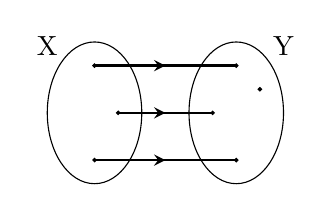
\begin{tikzpicture}[scale=0.3]
    \draw (2,3) ellipse (2cm and 3cm);
    \draw (8,3) ellipse (2cm and 3cm);

    \draw (0,5) node[above]{X};
    \draw (10,5) node[above]{Y};

    \filldraw[black] (2,5) circle (2pt);
    \filldraw[black] (8,5) circle (2pt);
    \draw[thick] (2,5) -- (8,5);
    \draw[-stealth, thick] (2,5) -- (5,5);

    \filldraw[black] (3,3) circle (2pt);
    \filldraw[black] (7,3) circle (2pt);
    \draw[thick] (3,3) -- (7,3);
    \draw[-stealth, thick] (3,3) -- (5,3);

    \filldraw[black] (2,1) circle (2pt);
    \filldraw[black] (8,1) circle (2pt);
    \draw[thick] (2,1) -- (8,1);
    \draw[-stealth, thick] (2,1) -- (5,1);

    \filldraw[black] (9,4) circle (2pt);
\end{tikzpicture}}\parbox{\textwidth - 4cm}{
    тобто різні елементи мають різні образи.
}

--- сюрєктивне(сюрєкція), якщо $f(X) = Y$

\noindent\parbox{4cm}{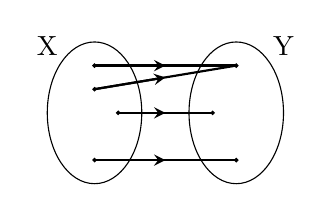
\begin{tikzpicture}[scale=0.3]
    \draw (2,3) ellipse (2cm and 3cm);
    \draw (8,3) ellipse (2cm and 3cm);

    \draw (0,5) node[above]{X};
    \draw (10,5) node[above]{Y};

    \filldraw[black] (2,5) circle (2pt);
    \filldraw[black] (8,5) circle (2pt);
    \draw[thick] (2,5) -- (8,5);
    \draw[-stealth, thick] (2,5) -- (5,5);
    \filldraw[black] (2,4) circle (2pt);
    \draw[thick] (2,4) -- (8,5);
    \draw[-stealth, thick] (2,4) -- (5,4.5);

    \filldraw[black] (3,3) circle (2pt);
    \filldraw[black] (7,3) circle (2pt);
    \draw[thick] (3,3) -- (7,3);
    \draw[-stealth, thick] (3,3) -- (5,3);

    \filldraw[black] (2,1) circle (2pt);
    \filldraw[black] (8,1) circle (2pt);
    \draw[thick] (2,1) -- (8,1);
    \draw[-stealth, thick] (2,1) -- (5,1);
\end{tikzpicture}}\parbox{\textwidth - 4cm}{
    (повний образ всього $X$ є в $Y$, тобто в $Y$ немає вільних елементів)
}

--- бієктивне(бієкція, взаємно однозначне відображення), якщо воно одночасно є сюрєкцією та інєкцією.

\noindent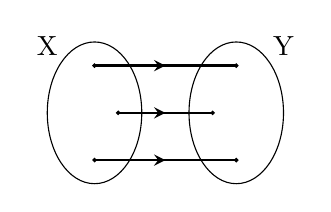
\begin{tikzpicture}[scale=0.3]
    \draw (2,3) ellipse (2cm and 3cm);
    \draw (8,3) ellipse (2cm and 3cm);

    \draw (0,5) node[above]{X};
    \draw (10,5) node[above]{Y};

    \filldraw[black] (2,5) circle (2pt);
    \filldraw[black] (8,5) circle (2pt);
    \draw[thick] (2,5) -- (8,5);
    \draw[-stealth, thick] (2,5) -- (5,5);

    \filldraw[black] (3,3) circle (2pt);
    \filldraw[black] (7,3) circle (2pt);
    \draw[thick] (3,3) -- (7,3);
    \draw[-stealth, thick] (3,3) -- (5,3);

    \filldraw[black] (2,1) circle (2pt);
    \filldraw[black] (8,1) circle (2pt);
    \draw[thick] (2,1) -- (8,1);
    \draw[-stealth, thick] (2,1) -- (5,1);
\end{tikzpicture}

--- загального виду -- ні сюрєктивне ні інєктивне.

\noindent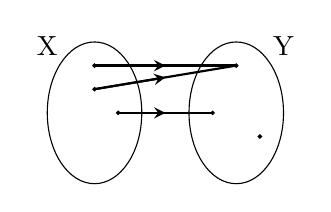
\begin{tikzpicture}[scale=0.3]
    \draw (2,3) ellipse (2cm and 3cm);
    \draw (8,3) ellipse (2cm and 3cm);

    \draw (0,5) node[above]{X};
    \draw (10,5) node[above]{Y};

    \filldraw[black] (2,5) circle (2pt);
    \filldraw[black] (8,5) circle (2pt);
    \draw[thick] (2,5) -- (8,5);
    \draw[-stealth, thick] (2,5) -- (5,5);
    \filldraw[black] (2,4) circle (2pt);
    \draw[thick] (2,4) -- (8,5);
    \draw[-stealth, thick] (2,4) -- (5,4.5);

    \filldraw[black] (3,3) circle (2pt);
    \filldraw[black] (7,3) circle (2pt);
    \draw[thick] (3,3) -- (7,3);
    \draw[-stealth, thick] (3,3) -- (5,3);

    \filldraw[black] (9,2) circle (2pt);
\end{tikzpicture}

\begin{definition}
    \textbf{Перестановка} або \textbf{перетворення} --- це бієкція множини на саму себе, тобто
    бієктивний оператор.
\end{definition}

\section{Зворотнє відображення та композиція відображень.}

